\section{Evaluation}


\subsection{Hypotheses}
We formulated three hypotheses.

\subsubsection{Hypothesis 1}
The uncorrected error rate to enter text using SwipeVR in virtual reality will be within 20\% of entering text on a smart phone keyboard in reality.

\subsubsection{Hypothesis 2}
More time is spent error correcting and editing than entering text.  Input mechanism should take this into account.

\subsubsection{Hypothesis 3}
SwipeVR is faster at editing and error correcting than smart phone keyboard in reality.

%\subsubsection{Hypothesis 4}
%Something about using multiple input mechanisms that don't conflict with each other. Error correction will not overlap in bandwidth with text entry.

We think that \textit{Hypothesis 1} will

We think that \textit{Hypothesis 2} will

We think that \textit{Hypothesis 3} holds as SwipeVR offers a tighter integrated between input devices and output displays used in smart phones.
The controllers in virtual reality are more \textit{expressive}~\cite{card1990design} than mobile phone keyboards.

\subsection{Participants}
X Y Z

\subsection{Apparatus}
Gaze keyboard\\
VR Controller Keyboard

\subsection{Procedure}
Each participant experimented with all apparatus.
Counter-balanced.
Each participant then proceeded for the test, which included 50 trials.
In 25 of the trials users were instructed to accurately input the phrase (including corrections if necessary) and in the remaining 25 trials participants were instructed to type without correcting the errors.
The data measured while the users were accurately typing the phrases vs. typing with no error correction were presented as corrected time and error rate and uncorrected accordingly.
The total number of trials each participant conducted is 180.
Data including user's actions and timing were logged and no timing or error rate information was visible to the participants during the study.
At the end of the experiment, participants filled out a questionnaire regarding their experiences with the different text entry methods and their preferences.

\subsection{Data Collection}
Input stream of insertions, deletion, edits that are analyzed for measures. Session number.

\subsection{Phrase Set}
We selected 50 phrases from a collection of 500 phrases commonly used for text entry evaluations~\cite{mackenzie2003phrase}.
The corpus doesn't include phrases with punctuation marks.  

We add five phrases with punctuation marks so the evaluation more closely mimics real-life interactions.
Non-alphanumeric symbols are rarely considered in text input research~\cite{mackenzie2003phrase} even though some punctuations (. - ' ( ) ") are more frequent than the least common English letter (q)~\cite{malikpunctuation}.
Moreover, the entry systems under evaluation use different interaction technique for punctuation then for characters.
Thus, this addition more fully tests the transition time between interaction techniques. 

Copying pre-selected phrase is usually the preferred method for text entry when doing evaluations in a lab setting~\cite{mackenzie2002character, mackenzie2003phrase}.
Although, entry rates should be regarded differently when the user is composing text instead instead of transcribing prompted phrases.
When the user composes text on their own, there could be substantial thinking time ~\cite{shneiderman2000limits} and other considerations that are difficult to measure.
Thus, sources of variation are present that could confound the  dependent variable.
We thus those to only use pre-selected phrases and rely on qualitative feedback to develop a holistic understanding for usability.

\subsection{Measures}
We use StreamAnalyzer~\cite{wobbrock2006analyzing} to  analyzes the text input stream logs created by TextTest~\cite{wobbrock2006analyzing} and produces text file output.
Besides parsing and analyzing batches of XML log files, StreamAnalyzer can also take presented strings and input streams typed directly on the console when run with the -d command line switch.


In the field of text entry, several metrics are used to characterize a method's performance ~\cite{wobbrock2007measures,arif2009analysis}.
Here, we discuss the most common performance metrics that we used to evaluate the  performance of each input devices.  


\subsubsection{Words per Minute}
Words per minute (~$WPM$) is perhaps the most widely reported empirical measure of
text entry performance~\cite{wobbrock2007measures}:

\[ 
WPM={\vert T\vert -1\over S}\times 60\times{1\over 5}. \eqno{\hbox{(1)}}
\]

Where, $S$ is the time in seconds from the first key press to the last, which means that the entry of the first character is never timed, which is the motivation for the "- 1" in the numerator of (1)~\cite{yamada1980historical}.
English words by convention are treated as having five characters~\cite{yamada1980historical}.

\subsubsection{Error Rate}
Error Rate (~$ER$) is the ratio of the total number of incorrect characters in the transcribed text to the length of the transcribed text:

\[
ER={INF\over \vert T\vert }\times 100\%. \eqno{\hbox{(2)}}
\]

Where, Incorrect Not Fixed (~$INF$) is the number of unnoticed incorrect characters in the transcribed text.

\subsubsection{Subjective }
we ask the user to evaluate each entry mechanism on a 5-point Likert Scale (Strongly Disagree, Disagree, neutral, Agree, Strongly Agree).
Additionally, users are  interviewed to further understand the their qualitative experience.

\subsubsection{Performance}
The input device felt responsive\\
The visuals were smooth and didn't freeze\\
The input device worked properly\\
The system was over responsive and showed inputs that I didn't enter\\
The system was under responsive and didn't showed inputs that I thought I entered

\subsubsection{Design}
It is easy to understand what to do with the input device\\
It was easy to learn how to use the input device\\
The interface was intuitive\\
This application has a graphical interface pleasant and understandable\\
The text and input were clearly visible

\subsubsection{Ergonomics}
I felt arm strain\\
I felt hand strain\\
I felt hand Nausea\\
I felt dizzy when using the system\\
I felt nauseous when using the system

\subsubsection{Applications}
I would use the input device to do a web search\\
I would use the input device to write an email\\
I would use the input device in public\\
I would use the input device at home\\
I would use the input device at a park\\
I would use the input device to chat (text)\\
I would use the input device to edit a letter

\subsection{Experiment A: Speed Without Corrections}
~\cite{william1995theoretical}

\subsection{Experiment B: Learnability}
We repeated each experiment 5 times each users and measured the delta across sessions to determine the learnaniltiy of the method.

\subsubsection{Experiment C: Error Rate Of Each Device}
The independent variable in the experiment was the interaction technique used. Dependent variables were time for task completion (dependent on word/phrase length), number of correct characters typed per minute (independent of word/phrase length), number of typing errors. Time for task completion was
measured automatically by the system, and the number of
characters in the wordphrase was divided by this value to
obtain the characters per minute measure. The number of
errors was recorded manually. Comfort ratings were each on a
ten-point scale, and were obtained at the beginning of the
experiment and after each set of trials. 

\subsection{Experiment C: Error Correction Time and Accuracy}






\begin{figure}
\centering
\begin{tikzpicture}
\begin{axis}[
    title=Box Plot of Total Error Rate,
	boxplot/draw direction=y,
  xtick={1,2,3,4},
  xticklabels={Speech, Gaze, Mobile, SwipeVR},
]

\addplot+[boxplot prepared={
  lower whisker=2.5,
  lower quartile=4,
  median=8.5,
  upper quartile=12,
  upper whisker=15}
]
coordinates {};

\addplot+[boxplot prepared={
  lower whisker=2.5, 
  lower quartile=3,
  median=8.5, 
  upper quartile=12,
  upper whisker=15}
]
coordinates {};

\addplot+[boxplot prepared={
  draw position=3,
  lower whisker=2.5,
  lower quartile=4,
  median=8.5,
  upper quartile=12,
  upper whisker=15}
]
coordinates {};

\addplot+[boxplot prepared={
  draw position=4,
  lower whisker=2.5,
  lower quartile=4,
  median=8.5,
  upper quartile=12,
  upper whisker=15}
]
coordinates {};


\end{axis}
\end{tikzpicture}



	\caption{Total error rate as a function of language and input method.}
  ~\label{fig:graphErrorRate}
\end{figure}




\begin{figure}
\centering
	\begin{tikzpicture}[scale=.6]

     	\pie{8/Thinking, 28/Composing, 22/Error Correcting, 42/Editing}[explode=0.1]
	\end{tikzpicture}
	\caption{Absolute distance finger moved vs. time vs. buffer.}
	~\label{fig:distance}
	\end{figure}

\begin{figure}
\centering
	\begin{tikzpicture}[scale=.6]

     	\pie{8/Thinking, 28/Composing, 22/Error Correcting, 42/Editing}[explode=0.1]
	\end{tikzpicture}
	\caption{Time proportion of users' time spent entering vs error correcting.}
	~\label{fig:graphPercenTime}
	\end{figure}

\begin{figure}
\centering
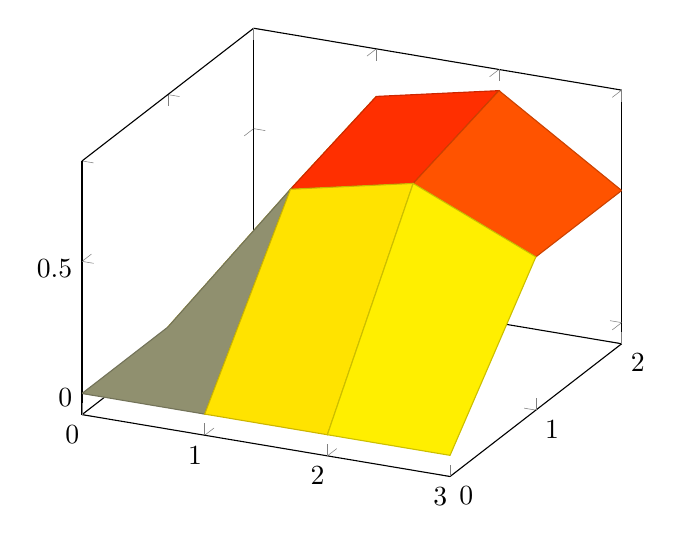
\begin{tikzpicture}
\begin{axis}
% this yields also a 3x4 matrix:
\addplot3[surf,mesh/rows=3] coordinates {
(0,0,0) (1,0,0) (2,0,0) (3,0,0)
(0,1,0) (1,1,0.6) (2,1,0.7) (3,1,0.5)
(0,2,0) (1,2,0.7) (2,2,0.8) (3,2,0.5)
};
\end{axis}
\end{tikzpicture}


	\caption{(Bar graph of arm strain, hand strain, neck strain, dizziness/nausea)  Differences between the initial and final subjective comfort ratings for each of the four techniques in the experiment 
}~\label{fig:graphLearning}
\end{figure}

\begin{figure}
\centering

	
\includegraphics[width=0.9\columnwidth]{figures/sigchi-logo}

	\caption{(Participants' subjective evaluation of difficulty 
}~\label{fig:graphLikert}
\end{figure}


\section{Results}

learning curve and extrapolated learning curve shown in Figure~\ref{fig:learnability}.
These are fit according to a power law and allow us to speculate about performance in future sessions.

SwipeVR allows for the user to enter text at 34 WPM.

See Table~\ref{tab:tableResults}\\
See Figure~\ref{fig:graphWPM}\\
See Figure~\ref{fig:graphErrorRate}\\
See Figure~\ref{fig:graphPercenTime}\\

\section{Discussion}
We argue that we have confirmed H1, H2, and H3.

Concerning H1 (SwipeVR faster than gaze), we find there are significant differences between text entry rates of both approaches.

